%interno poro�ilo
%\documentclass[internal, slovene]{FRIreport}

%zaklju�no poro�ilo
%\documentclass[slovene]{FRIreport}

%seminarska naloga
\documentclass[seminar, slovene]{FRIreport}

% AMS fonts required
\usepackage{iopams}  

% package to include graphics in ps, eps or png format
\usepackage{graphicx}
\usepackage{epstopdf}
% the graphics path
\graphicspath{{img/}}

% define equation referencing
\newcommand{\eqref}[1]{(\ref{#1})}

% define figure referencing
\newcommand{\figref}[1]{\ref{#1}}

% define real numbers symbol
\newcommand{\Rset}{\ensuremath{\mathbb{R}}} 
\newcommand{\R}{\Rset} 
% define natural numbers symbol
\newcommand{\Nset}{\ensuremath{\mathbb{N}}} 
\newcommand{\N}{\Nset} 
% define euclidean vector space symbol
\newcommand{\Eset}{\ensuremath{\mathbb{E}}} 
\newcommand{\E}{\Eset} 

\newcommand{\imp}[1]{{\color{P654M}#1\normalcolor}}

%%%
\newcommand{\angl}[1]{(\textit{angl.} #1)}


\usepackage{tikz}
\usetikzlibrary{shapes.gates.logic.US}
\usetikzlibrary{circuits.logic.US}
\usepackage{circuitikz}

\newenvironment{vezje}{
\pgfkeys{
	and/.style={draw, very thin, minimum size=0.6cm, on chain=trak},
	%nadzorna enota
	head/.style={draw, minimum width=2cm, minimum height=1.2cm}
}
\begin{tikzpicture}}{\end{tikzpicture}}


%main
\begin{document}

\title{QCA sekven\v cna ALE}

\author{Miha Zidar, Anže Pečar, Matic Potočnik, Željko Plesac, Jan Varljen}

%\address{Skupina 1}

\begin{abstract}
V seminarju bomo opisali zasnovo sekvenčne ALE s kvantnimi celičnimi avtomati, z uporabo programa QCAdesigner.

\Keywords{kvantni celični avtomati, aritmetično-logična enota, modeliranje in simulacija}
\end{abstract}

%
%%
\section{Uvod}
Predvideva se, da bo že čez nekaj desetletij minituarizacija in zmogljivost čipov, grajenih na siliciju, dosegla končno stopnjo in bo potrebno za večjo procesno moč preiti na drug osnovni material in najverjetneje tudi zelo spremeniti pristop k modeliranju vezij. Ena izmed obetajočih alternativ so kvantni celični avtomati \angl{quantum cellular automata -- QCA}, ki obljubljajo mnoge prednosti pred klasičinimi vezji:
\begin{itemize}
\item Možnost večnivojskih vezij
\item Možnost križanja vodil
\item Enostavna realizacija nekaterih časovnih vezij
\item Potencialno nižja poraba in višji takt delovanja
\item $\dots$
\end{itemize}
V tem seminarju bomo opisali zasnovo sekvenčne ALE, ki smo jo modelirali z uporabo odprtokodnega programa QCADesigner\cite{walus:2004} (za skice logičnih vezij smo uporabili TinyCAD). Sekvenčnost enote tu pomeni, da enota načeloma ne izvaja operacij nad vsebino končno dolgih registrov, ampak sprejema tok(sekvenco) bitov, nad posameznimi biti izvaja operacije in tudi svoj izhod podaja kot tok bitov. Kot bomo videli v nadaljevanju, to za določene operacije ni možno in jih interno še vedno realiziramo z registri. Za večino osnovnih operacij pa je sekvenčna implementacija možna in se lepo prilega realizaciji s QCA-ji.

%
%%
\section{Metode}
V tem odseku bomo predstavili nekatere odločitve in metode snovanja, ki smo jih uporabili pri zasnovi naše ALE.

\subsection{Osnovni opis ALE}
Implementirali smo logično poln sistem operacij. Za izbiro operacije smo uporabili tri bite. Naša ALE bo podpirala naslednje operacije: (NI ŠE PRAVA TABELA!)

\begin{center}
\begin{tabular}{ | c | c | c | }\hline
\textbf{Operacija} & \textbf{Oznaka} & \textbf{Operacijska koda} \\ \hline
NOP & $\varnothing$ & 0 0 0 \\
NOT & $\lnot$ & 0 0 1 \\
AND & $\wedge$ & 0 1 0 \\
OR & $\vee$ & 0 1 1 \\
ADD & $+$ & 1 0 0 \\
SUB & $-$ & 1 0 1 \\
MUL & $\times$ & 1 1 0 \\
DIV & $\div$ & 1 1 1 \\ \hline
\end{tabular}
\end{center}

%
%%
\section{Rezultati}
\subsection{Izbira operacije}
\begin{figure}[htb]
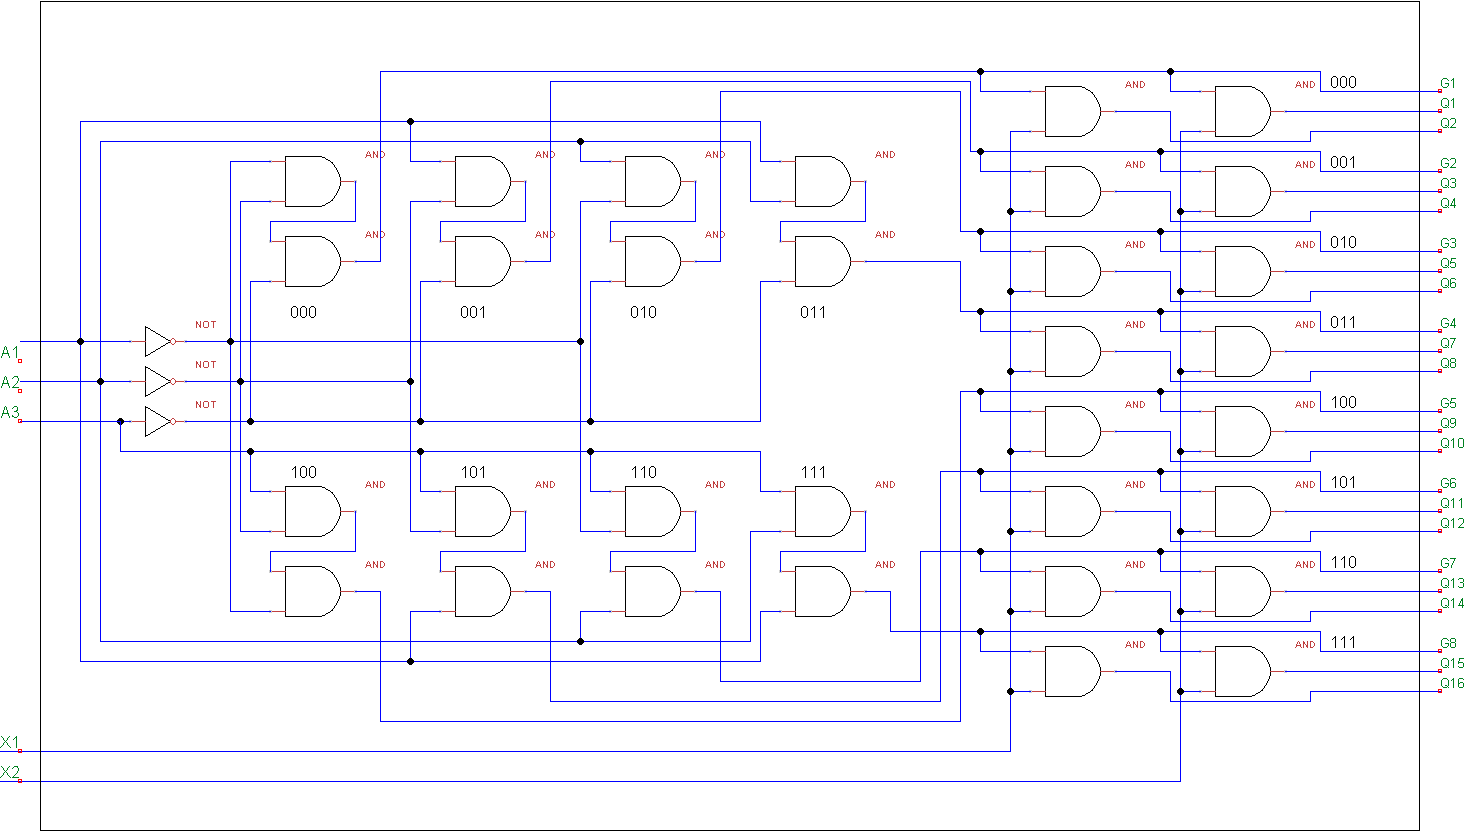
\includegraphics[width=15cm]{vezja/img/demux.png}
\caption{Demultiplekser}
\label{demux}
\end{figure}
\pagebreak

\subsection{Seštevalnik}
\begin{figure}[htb]
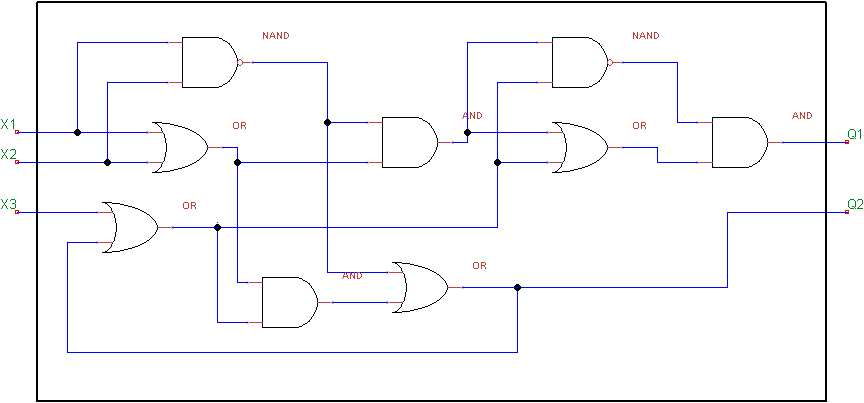
\includegraphics[width=14cm]{vezja/img/sestevalnik.png}
\caption{Seštevalnik}
\label{sestevalnik}
\end{figure}
\pagebreak

%
%%
\section{Zaključek}
Zaključki z nekaj izhodišči za nadaljnje delo.

%
%%
\References
\bibliographystyle{elsart-num-sl}
\bibliography{sample}

\end{document}
